\documentclass[tikz]{standalone}

\usetikzlibrary{arrows}
\usetikzlibrary{arrows.meta}

\begin{document}

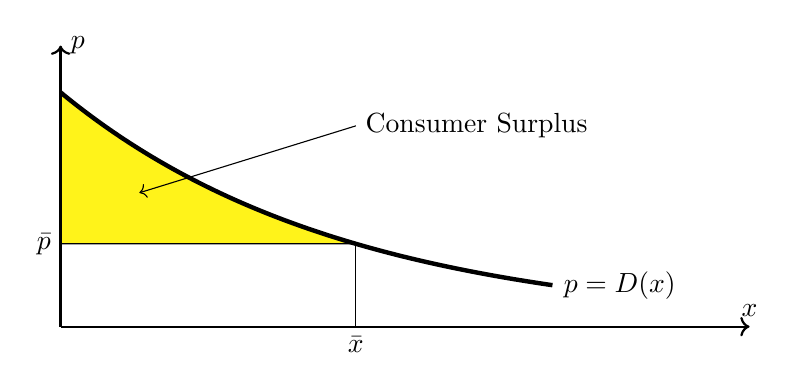
\begin{tikzpicture}[xscale=2.5,yscale=0.85]

    % shade region
    \draw[fill=yellow!90] plot[smooth, samples=10, domain=0:1.5] (\x,3.5/2^\x) |- (0,1.237) -- cycle;
      
    % draw axes 
    \draw[thick,->] (0,0) -- (3.5,0) node[above] {$x$};
    \draw[thick,->] (0,0) -- (0,4.2) node[right] {$p$};
      
    % draw curve
    \draw[ultra thick,domain=0:2.5,samples = 100, smooth,variable=\x,black] plot ({\x},{3.5/2^\x})node[right] {$p=D(x)$};
  
    \draw (1.5,1.237) -- (1.5,0) node[below] {$\bar{x}$};
    \draw (1.5,1.237) -- (0,1.237) node[left] {$\bar{p}$};
    \draw[<-] (0.4,2) -- (1.5,3) node[right] {Consumer Surplus};
  \end{tikzpicture}
  

  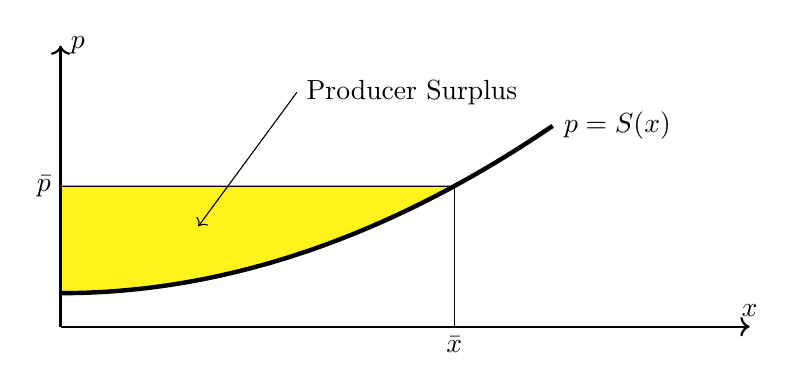
\begin{tikzpicture}[xscale=2.5,yscale=0.85]
    % shade region
    \draw[fill=yellow!90] plot[smooth, samples=100, domain=0:2] (\x,0.5+0.4*\x*\x) -| (0,0.5) ;
  
    % draw axes 
    \draw[thick,->] (0,0) -- (3.5,0) node[above] {$x$};
    \draw[thick,->] (0,0) -- (0,4.2) node[right] {$p$};
  
    % draw curves
    \draw[ultra thick,domain=0:2.5,smooth,variable=\x,black] plot ({\x},{0.5+0.4*\x*\x}) node[right] {$p=S(x)$};
  
    \draw (2,2.1) -- (2,0) node[below] {$\bar{x}$};
    \draw (2,2.1) -- (0,2.1) node[left] {$\bar{p}$};
    \draw[<-] (0.7,1.5)--(1.2,3.5) node[right] {Producer Surplus};
  
  \end{tikzpicture}

  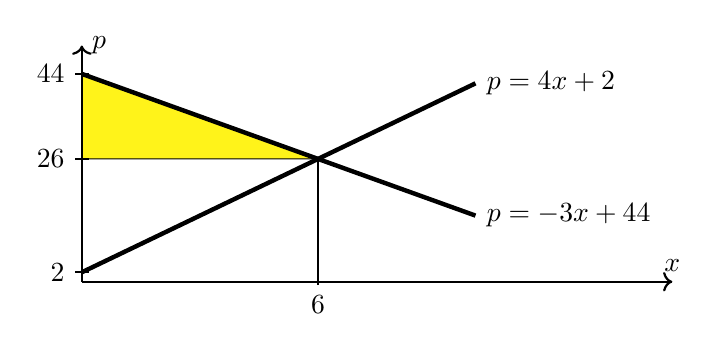
\begin{tikzpicture}[scale=0.5,yscale=0.12]

    % \draw[fill=white] (-2,-10) rectangle ++(19,70);
  
    % shade region
    \draw[fill=yellow!90] plot[smooth, samples=10, domain=0:6] (\x,44 - 3*\x) -| (0,44);
      
    % draw axes 
    \draw[thick,->] (0,0) -- (15,0) node[above] {$x$};
    \draw[thick,->] (0,0) -- (0,50) node[right] {$p$};
      
    % draw curve
    \draw[ultra thick,domain=0:10,samples = 100, smooth,variable=\x,black] plot ({\x},{44 - 3*\x}) node[right] {$p=-3x+44$};
    \draw[ultra thick,domain=0:10,samples = 100, smooth,variable=\x,black] plot ({\x},{2 + 4*\x}) node[right] {$p=4x+2$};
  
    % tick marks
    \foreach \x in {6} 
      \draw [thick] (\x cm,20pt) -- (\x cm,-20pt) node[below] {\x};
    \foreach \y in {2,26,44} 
      \draw [thick] (5pt,\y cm) -- (-5pt,\y cm) node[left] {\y};
  
    \draw (6,26) -- (6,0);
    %      \draw (6,26) -- (0,26) node[left] {$\bar{p}$};
    %      %\draw[<-] (0.4,2) -- (1.5,3) node[right] {Consumer Surplus};
  \end{tikzpicture}

  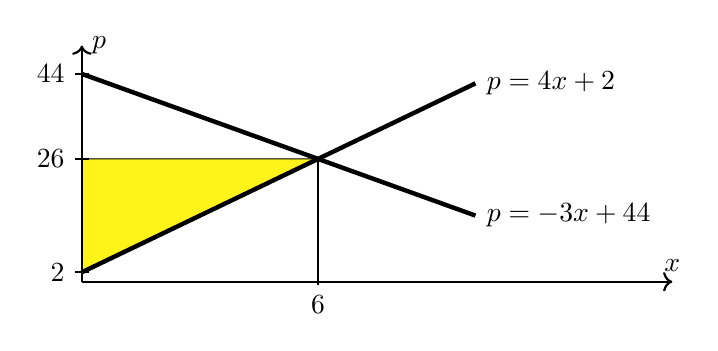
\begin{tikzpicture}[scale = 0.5,yscale=0.12]

    % \draw[fill=white] (-2,-10) rectangle ++(19,70);
  
    % shade region
    \draw[fill=yellow!90] plot[smooth, samples=10, domain=0:6] (\x,2 + 4*\x) -| (0,2);
      
    % draw axes 
    \draw[thick,->] (0,0) -- (15,0) node[above] {$x$};
    \draw[thick,->] (0,0) -- (0,50) node[right] {$p$};
      
    % draw curve
    \draw[ultra thick,domain=0:10,samples = 100, smooth,variable=\x,black] plot ({\x},{44 - 3*\x}) node[right] {$p=-3x+44$};
    \draw[ultra thick,domain=0:10,samples = 100, smooth,variable=\x,black] plot ({\x},{2 + 4*\x}) node[right] {$p=4x+2$};
  
    % tick marks
    \foreach \x in {6} 
      \draw [thick] (\x cm,20pt) -- (\x cm,-20pt) node[below] {\x};
    \foreach \y in {2,26,44} 
      \draw [thick] (5pt,\y cm) -- (-5pt,\y cm) node[left] {\y};
  
    \draw (6,26) -- (6,0);
    %      \draw (6,26) -- (0,26) node[left] {$\bar{p}$};
    %      %\draw[<-] (0.4,2) -- (1.5,3) node[right] {Consumer Surplus};
  \end{tikzpicture}

  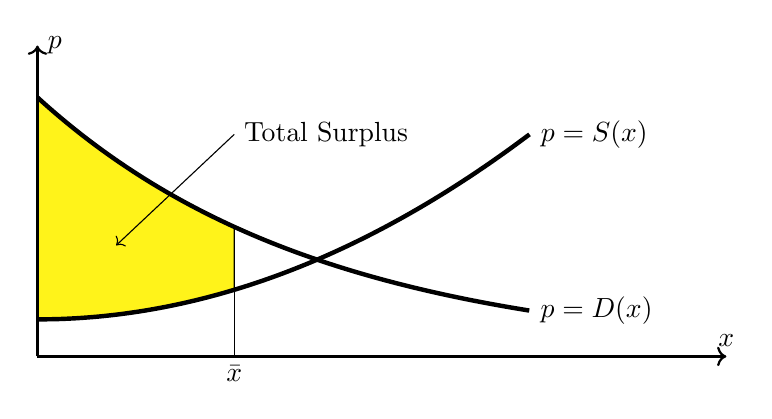
\begin{tikzpicture}[xscale=2.5,yscale=0.94]

    % shade region
    \draw[fill=yellow!90] plot[smooth, samples=10, domain=0:1] (\x,3.5/2^\x) -- 
    plot[smooth, samples=100, domain=1:0] (\x,0.5+0.4*\x*\x);
  
    % draw axes 
    \draw[thick,->] (0,0) -- (3.5,0) node[above] {$x$};
    \draw[thick,->] (0,0) -- (0,4.2) node[right] {$p$};
      
    % draw curves
    \draw[ultra thick,domain=0:2.5,samples = 100, smooth,variable=\x,black] plot ({\x},{3.5/2^\x})node[right] {$p=D(x)$};
    \draw[ultra thick,domain=0:2.5,smooth,variable=\x,black] plot ({\x},{0.5+0.4*\x*\x}) node[right] {$p=S(x)$};
  
    % draw labels
    \draw (1,0.9) -- (1,0) node[below] {$\bar{x}$};
    \draw[<-] (0.4,1.5) -- (1,3) node[right] {Total Surplus};
  \end{tikzpicture}

  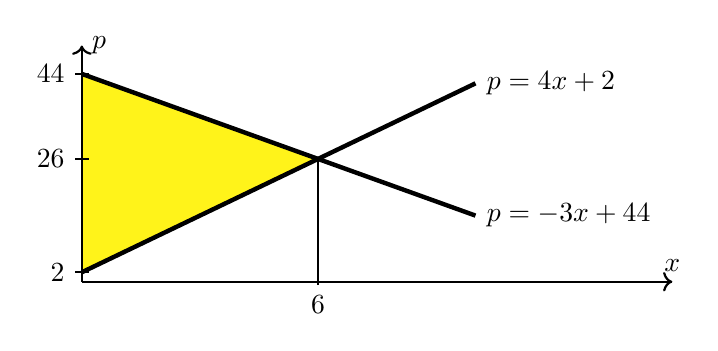
\begin{tikzpicture}[scale = 0.5,yscale=0.12]

    % \draw[fill=white] (-2,-10) rectangle ++(19,70);
  
    % shade region
    \draw[fill=yellow!90] 
    plot[smooth, samples=10, domain=0:6] (\x,44 - 3*\x) --
    plot[smooth, samples=10, domain=6:0] (\x,2 + 4*\x) -- cycle;
      
    % draw axes 
    \draw[thick,->] (0,0) -- (15,0) node[above] {$x$};
    \draw[thick,->] (0,0) -- (0,50) node[right] {$p$};
      
    % draw curve
    \draw[ultra thick,domain=0:10,samples = 100, smooth,variable=\x,black] plot ({\x},{44 - 3*\x}) node[right] {$p=-3x+44$};
    \draw[ultra thick,domain=0:10,samples = 100, smooth,variable=\x,black] plot ({\x},{2 + 4*\x}) node[right] {$p=4x+2$};
  
    % tick marks
    \foreach \x in {6} 
      \draw [thick] (\x cm,20pt) -- (\x cm,-20pt) node[below] {\x};
    \foreach \y in {2,26,44} 
      \draw [thick] (5pt,\y cm) -- (-5pt,\y cm) node[left] {\y};
  
    \draw (6,26) -- (6,0);
    %      \draw (6,26) -- (0,26) node[left] {$\bar{p}$};
    %      %\draw[<-] (0.4,2) -- (1.5,3) node[right] {Consumer Surplus};
  \end{tikzpicture}
  


\end{document} 